\documentclass{slnotes}

\begin{document}
\chapter{Powers of 2}
\begin{tabular}{llll}
\toprule
\(n\) & \(2^n\) & \(n\) & \(2^n\) \tabularnewline
\midrule
-10 & 0.0009765625 & 1 & 2 \tabularnewline
-9  & 0.001953125  & 2 & 4 \tabularnewline
-8  & 0.00390625   & 3 & 8 \tabularnewline
-7  & 0.0078125    & 4 & 16 \tabularnewline
-6  & 0.015625     & 5 & 32 \tabularnewline
-5  & 0.03125      & 6 & 64 \tabularnewline
-4  & 0.0625       & 7 & 128 \tabularnewline
-3  & 0.125        & 8 & 256 \tabularnewline
-2  & 0.25         & 9 & 512 \tabularnewline
-1  & 0.5          & 10 & 1024 \tabularnewline
15 & 32768         & 16 & 65536 \tabularnewline
20 & 1048576       & 24 & 16777216 \tabularnewline
30 & 1073741824 \tabularnewline
31 & 2147483648    & 32 & 4294967296 \tabularnewline
\bottomrule
\end{tabular}
\chapter{Number systems}
\(n\) bits can represent \(2^n\) values.

To convert a decimal to binary, divide by 2 repeatedly; the remainders form the answer, with the first being the LSB. To convert a fraction to binary, multiply by 2 repeatedly; the carries form the answer, with the first being the MSB.

\sldef{Sign-and-magnitude}. One bit for sign, remaining bits for magnitude. Range is \([-(2^{n-1}-1), 2^{n-1}-1]\). Two zeroes. To negate, flip sign bit.

\sldef{1's complement}. MSB is sign. Range is same as above. Two zeroes. To negate, flip all bits: \(-x = 2^n - x - 1\). When adding, if there is a carry out of MSB, add 1 to the result.

\sldef{2's complement}. MSB is sign. Range is \([-2^{n-1}, 2^{n-1}-1]\). Only one zero. To negate, flip all bits and add 1: \(-x = 2^n - x\). When adding, ignore carry out of MSB.

Overflow has occurred if the operands have the same sign but the result has a different sign.

\sldef{Excess}. Excess-\(n\) means \(-n\) is represented as 0, etc.

\sldef{IEEE-754}. 32-bit: 1-bit sign, 8-bit exponent (excess-127), 23-bit mantissa. 64-bit: 1-bit sign, 11-bit exponent (excess-1023), 52-bit mantissa. When the exponent field is all 0, the mantissa is denormalised, and the actual exponent is the bias plus 1 (i.e. \(-126\) for 32-bit).
\chapter{MIPS}
\tablehead{\toprule Pseudo & Realised\tabularnewline}
\begin{xtabular}{ll}
\midrule
\code{move \$x, \$y} & \code{add \$x, \$y, \$zero}\tabularnewline
\midrule
\code{li \$x, 0xXXXXYYYY} & \begin{tabular}{@{}l@{}}\code{lui \$at, 0xXXXX} \tabularnewline
\code{ori \$x, \$at, 0xYYYY}\end{tabular}\tabularnewline
\midrule
\code{blt \$x, \$y, z} & \begin{tabular}{@{}l@{}}\code{slt \$t, \$x, \$y} \tabularnewline
\code{bne \$t, \$zero, z}\end{tabular}\tabularnewline
\midrule
\code{bgt \$x, \$y, z} & \begin{tabular}{@{}l@{}}\code{slt \$t, \$y, \$x} \tabularnewline
\code{bne \$t, \$zero, z}\end{tabular}\tabularnewline
\midrule
\code{ble \$x, \$y, z} & \begin{tabular}{@{}l@{}}\code{slt \$t, \$y, \$x} \tabularnewline
\code{beq \$t, \$zero, z}\end{tabular}\tabularnewline
\midrule
\code{bge \$x, \$y, z} & \begin{tabular}{@{}l@{}}\code{slt \$t, \$x, \$y} \tabularnewline
\code{beq \$t, \$zero, z}\end{tabular}\tabularnewline
\bottomrule
\end{xtabular}

To NOT \code{\$x}: \code{nor \$x, \$x, \$zero}.

XOR is R-format, \code{R[rd] = R[rs] \^{} R[rt]}, opcode 0, function 0x26.

\sldef{Control}. 1: \code{Reg\-Dst}, 2: \code{ALU\-Src}, 3: \code{Mem\-To\-Reg}, 4: \code{Reg\-Write}, 5: \code{Mem\-Read}, 6: \code{Mem\-Write}, 7: \code{Branch}, 8: \code{ALU\-op}.

\begin{tabular}{lllllllll}
\toprule
&1&2&3&4&5&6&7&8\tabularnewline
\midrule
R-type & 1 & 0 & 0 & 1 & 0 & 0 & 0 & 10 \tabularnewline
\code{lw} & 0 & 1 & 1 & 1 & 1 & 0 & 0 & 00 \tabularnewline
\code{sw} & X & 1 & X & 0 & 0 & 1 & 0 & 00 \tabularnewline
\code{beq} & X & 0 & X & 0 & 0 & 0 & 1 & 01 \tabularnewline
\bottomrule
\end{tabular}

\sldef{ALU control}. And: 0000. Or: 0001. Add: 0010. Subtract: 0110. SLT: 0111. NOR: 1100.

\onecolumn
\chapter{Datapath}
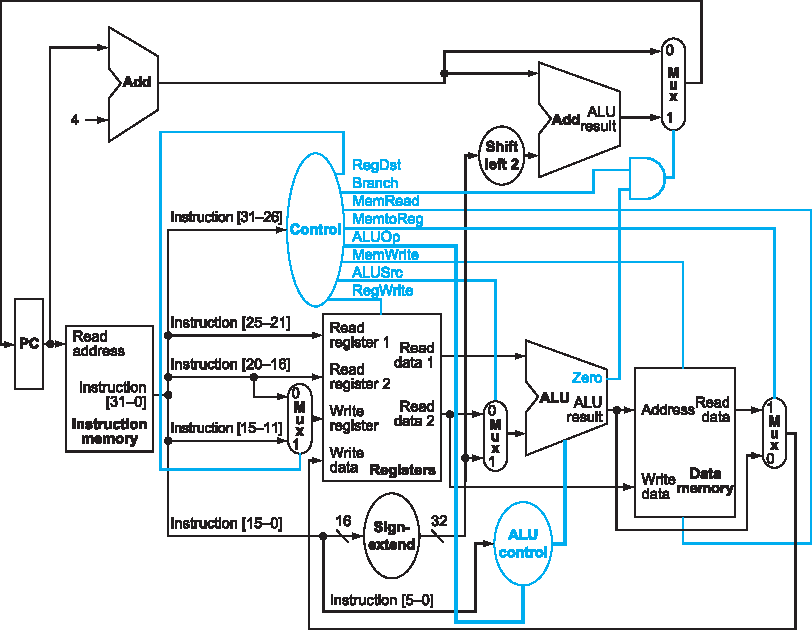
\includegraphics[width=\textwidth]{simple-mips-datapath.pdf}
\end{document}
